% vim:set et sts=2 sw=2 ts=2 tw=72:

\section{Introduction}

Between 50k and 70k commits are added to the Linux kernel per version,
requiring maintainers of older versions of the kernel to sift through
thousands of commits and merges with tools that are unable to filter and
effectively visualize projects at the scale of the kernel. Older
versions of the kernel are used in embedded systems and mobile phones;
for security purposes, performance needs, and changing hardware
requirements, maintainers must be able to understand the changes being
made in the current version of the kernel in order to produce the
necessary patches for the older versions of the kernel. Tools like Gitk
use a directed acyclic graph (DAG) model of the repository, showing all
commits and merges in chronological order by when the commit was
authored, not by when it arrived in the official Linux repository.

\begin{figure}
        \centering
        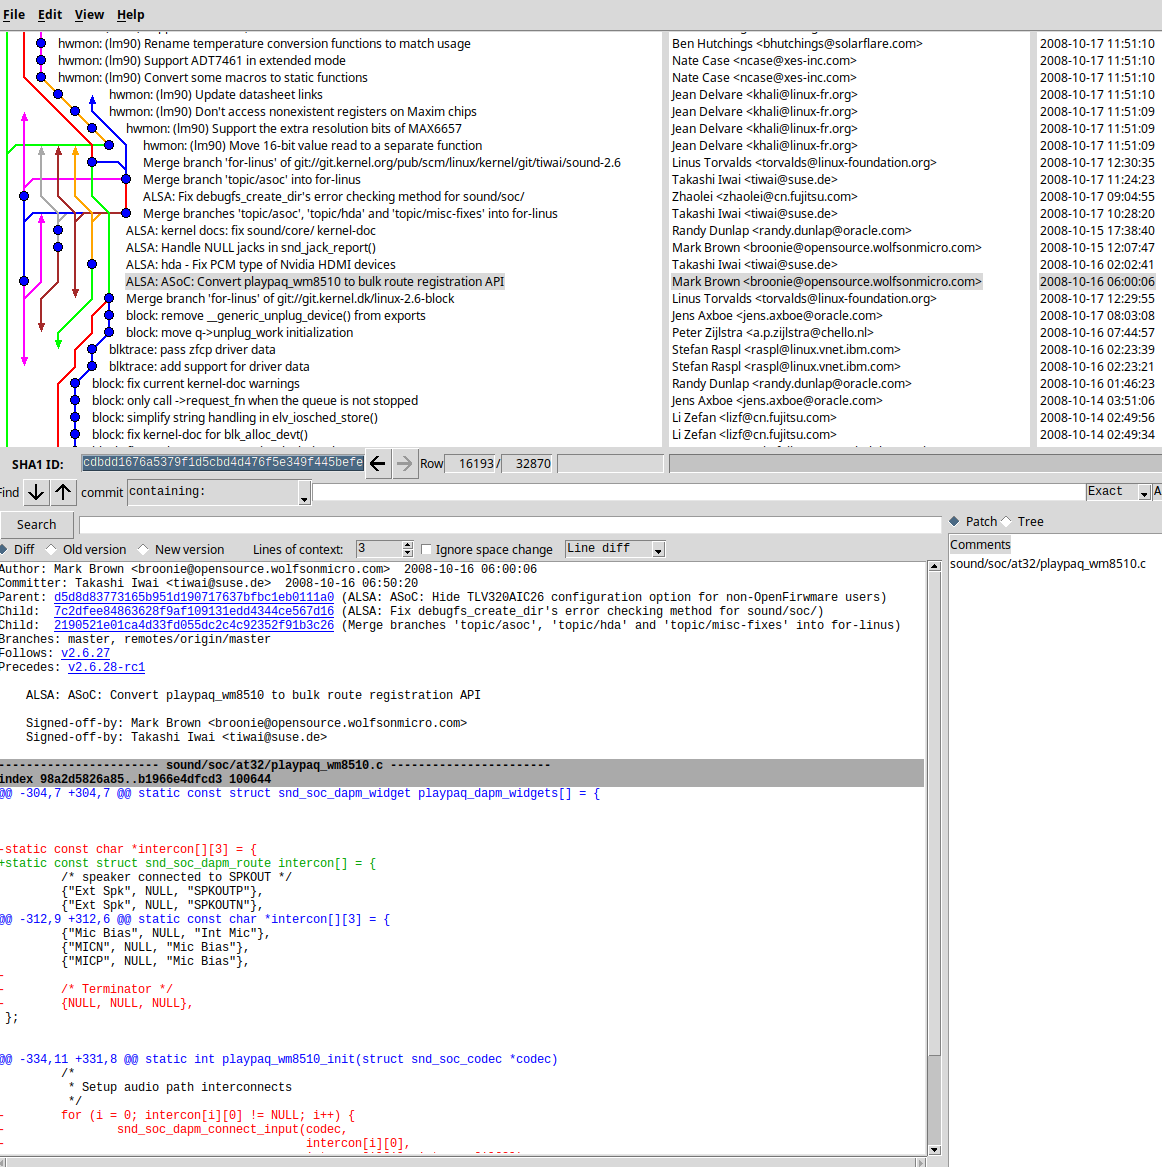
\includegraphics[width=0.97\linewidth]{figures/gitk.png}
        \caption{The Gitk interface centered on commit
          cdbdd1676a5379f1d5cbd4d476f5e349f445befe, \comB from the user
          study. The top-left pane shows the DAG and commit log preview,
          the top center pane shows the authors, and the top-right
          pane shows the commit dates. The bottom-left pane shows the
          full commit message, the parents and children of the commit,
          and the changes made to files in this commit. The bottom-right
          pane shows the list of the files modified by this commit.}
        \label{fig:gitk}
%\vspace{-4mm}
\end{figure}

\begin{figure}
        \centering
        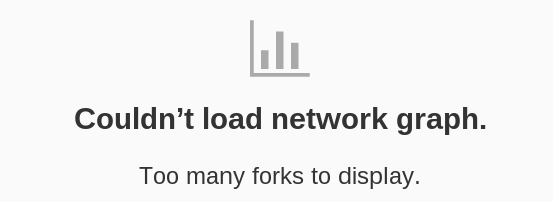
\includegraphics[width=0.8\linewidth]{figures/github_viewer.png}
        \caption{Github normally shows a visualization of the DAG,
          showing the commits, branches, and forks, but is unable to
          generate a visualization for projects at the size of the Linux
          repository.}
        \label{fig:gitfail}
%\vspace{-2mm}
\end{figure}

The DAG is able to provide a meaningful visualization in smaller
projects; it enables users to see when changes are made, when these
changes are merged, how each branch is interacting, and the point where
a branch forks from the master branch. In large modular projects, like
the Linux kernel, the DAG becomes a mess of merges and commits
(Figure~\ref{fig:gitk}) losing its visual meaning. In some cases, the
Linux kernel is simply too large for the system to generate a
visualization; Github provides a DAG view for a repository, but is
unable to display the visualization for projects at the scale of the
Linux of the kernel (Figure~\ref{fig:gitfail}). Between 60k and 70k new
commits are created for the Linux project every year; according to
previous work\cite{German2015}, a commit takes a median of 30 days from
the time it is authored until it arrives in the official repository. The
snapshot of the kernel tomorrow may be different than the snapshot from
today, containing new commits authored in the past; distinguishing these
new commits from the commits in the snapshot from today is not trivial.

One major challenge with visualizing the arrival of commits to a
repository is that Git does not store the date that a commit was merged
into another branch, including the master branch. To complicate the
problem, the DAG only has references to the ancestors of a commit (a
model necessary for the operation of Git), but maintainers would prefer
knowing the path a commit followed to reach the master repository.
Tracing a path that any commit followed to the master repository would
imply that for any given merge, it would be possible to know which
commits were merged. A user could inspect the commits that arrived into
the master branch within a given time-frame by checking which commits
were merged during that time-frame.

\dmg{add to the abstract an abbreviation of this sentence: see my comment in the abstract }
This paper makes three contributions; first, we describe a method of
converting the DAG of the Linux repository into the \mt of the
repository, that represents the path used by a commit to reach the
master branch; second, we present an implementation enabling the
inspection and visualization of merges in the Linux project using the
\mt modle; finally, we validate the \mt model and the implementation of
the visulization through a controlled user study. We further discuss the
issues of generalizing the model to other repositories, but present an
updated version that improves the performance of the algorithm by
pruning the DAG.\@

These methods and visualizations are implemented in a web-based tool
called \tool\footnote{\tool is currently available at
  \url{http://li.turingmachine.org}}. Our visualizations and tool
provide information about the location of any given commit or merge in
its respective merge-tree, the files edited, the modules edited, and the
commit message. \tool allows users to apply various filters, including
the release version, along with a keyword or phrase from the log
preview, the name of the author, or the commit hash. The user can
request all merges made by Linus that contain a commit or inner merge
that matches the search query, or just the commits and merges that match
the query.
